% The section about the agents' amount of the simulation itself
% @author Kalvin Döge
%

% graphics

\subsection{Anzahl aktiver Agenten}\label{subsec:activeagents}

Zur Bestimmung von der Anzahl an aktiven Agenten, wurde eine angenäherte Rechnung für die Population um die Alster genommen, da direkte Statistiken zur täglichen Anzahl an Verkehrsteilnehmern in Hamburg beziehungsweise in verschiedenen Stadtvierteln fehlen.
Um eine Annäherung an die Verkehrszahlen zu bekommen, wird zuerst die Verteilung über Haupt-, Neben- und Schwachverkehrszeiten untersucht.

Ein Arbeitstag, Montag bis Freitag, hat zwei große Hauptverkehrszeiten: morgens von 6 bis 9 Uhr und nachmittags von 15 bis 19 Uhr~\cite{FHH2015}.
In diesen beiden Zeiten werden die meisten Verkehrsteilnehmer auf den Straßen unterwegs sein und damit am ehesten Staus verursachen.

Die Nebenverkehrszeit tritt von 9 bis 15 Uhr~\cite{FHH2015} auf, die den Übergang zwischen den beiden Hauptverkehrszeiten darstellt.
Innerhalb dieser Zeit ist die Dichte an Verkehrsteilnehmern geringer als in der Hauptverkehrszeit, aber immer noch höher als in Schwachverkehrszeiten.

Die Schwachverkehrszeit ist von 20 Uhr bis 5 Uhr am nächsten Tag~\cite{FHH2015}, in der der Verkehr am geringsten ist, die Straßen leer und der Stau am seltensten auftritt.


Um den Verlauf über einen Tag nun mit zwei Hochpunkten und drei Tiefpunkten darzustellen, während dabei der zweite Tiefpunkt höher als der erste und dritte ist, lässt sich der grobe Verlauf über eine negierte Funktion 4.\ Grades darstellen.

\begin{figure}[h]
    \centering
    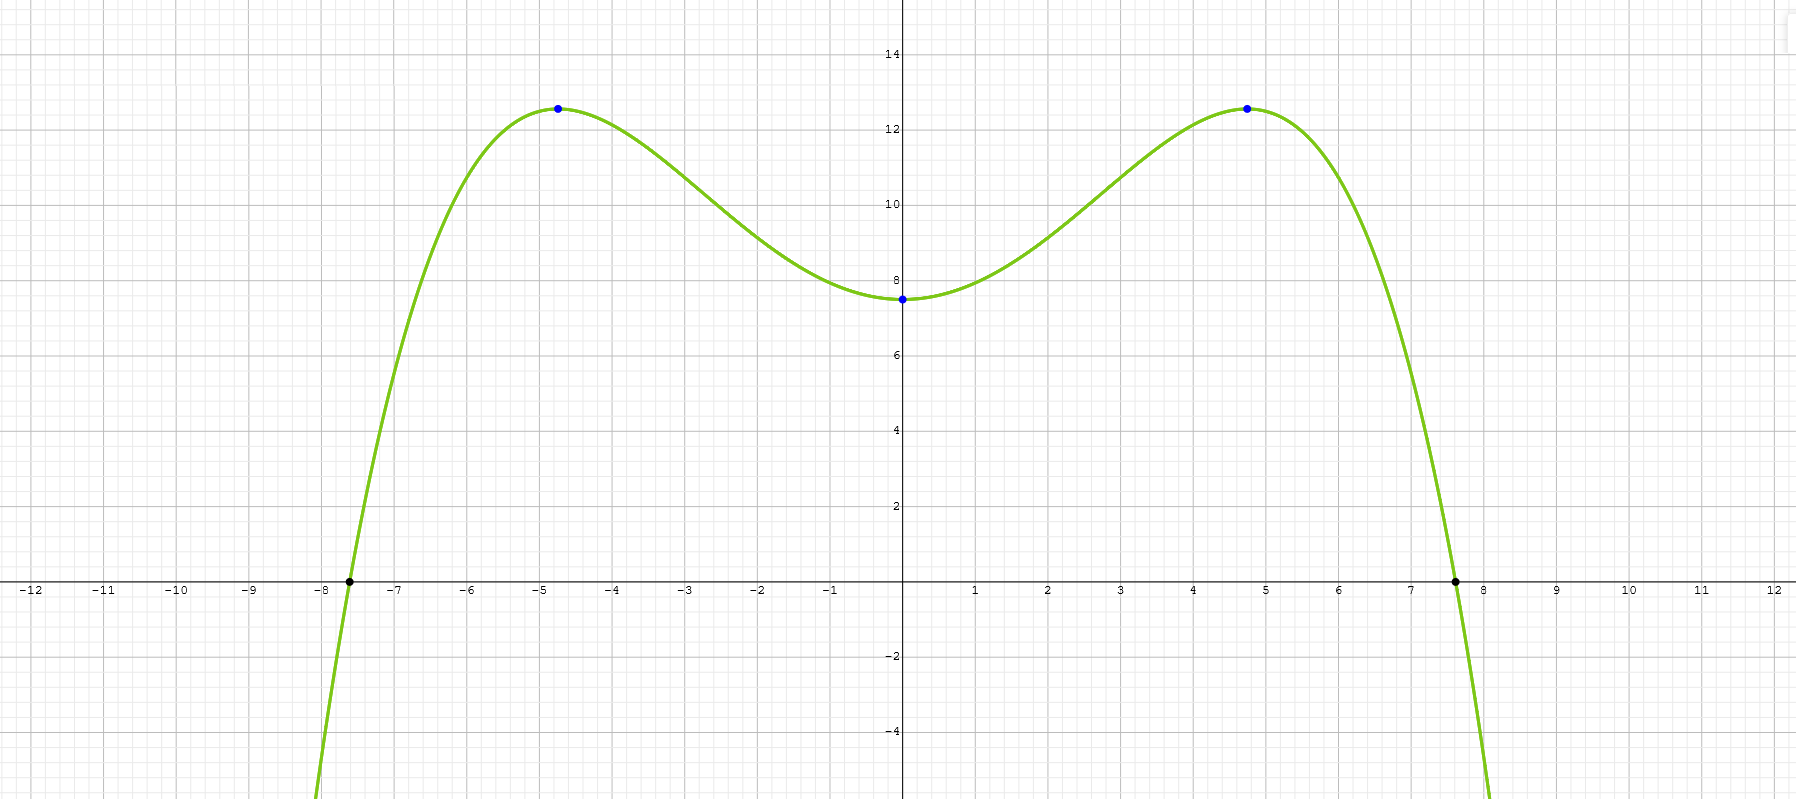
\includegraphics[width=1.00\textwidth]{poly-4-degree}
    \caption{Polynomialfunktion des 4. Grades zur Annäherung}
    \label{fig:poly-4-degree}
\end{figure}

Die Funktion aus der Grafik~\ref{fig:poly-4-degree} lautet: \[f(x)=-0.01x^4+0.45x^2+7.5\]

Die Grafik~\ref{fig:poly-4-degree} muss so interpretiert werden, als hätte die x-Achse eine Verschiebung von 12 Einheiten nach rechts noch erhalten, damit die Werte sich passend der Tagesstunden verteilen.
Entsprechend ist 0 Uhr hier bei x = -12, 12 Uhr ist bei x = 0 und 24 Uhr ist bei x = 12.

Zum Annähern selbst ist die Funktion aber nur ansatzweise nützlich, da wenn x die Stundenanzahl und f(x) der Prozentsatz aller aktiven Agenten darstellt, die Schwachverkehrszeiten bei einer Funktion 4.\ Grades auf der x-Achse in das Negative gehen würden.
Damit wäre aber, wenn f(x) Nullstellen bei \[x = -12, x = 12\] hätte, keine relativ gleiche Verteilung über die 9 Stunden, also wäre von 20 bis 5 Uhr keine relativ flache Schwachverkehrszeit.
Der zweite Ansatz wäre, bei einem anderen x-Wert die Nullstelle schneiden zu lassen, wie es in der Grafik~\ref{fig:poly-4-degree} zu sehen ist, also zum Beispiel an den Stellen \[x = -7.6, x = 7.6\]
x = -7.6 wäre um circa 4 Uhr und x = 7.6 wäre um circa 20 Uhr.
Bei diesem Ansatz werden dann aber negative Funktionswerten außerhalb der x-Werte auftreten und damit ,,negativen Verkehr`` verursachen.
Das kann logischerweise nicht in der realen Welt auftreten, also müssen die Werte auf 0 oder einen anderen Wert gesetzt werden.
Sollte der Wert auf 0 gesetzt werden, wäre das noch immer keine korrekte Darstellung für das Modell, da in der Schwachverkehrszeit noch immer Verkehr vorliegt.
Um einen besseren Funktionsverlauf zu gewährleisten, muss die Funktion interpoliert werden, um flachere Übergänge in die Schwachverkehrszeit zu bewerkstelligen.
Um den Verlauf beziehungsweise die Interpolation zu konstruieren, werden kubische Polynome genutzt, die an bekannten Punkten eine Ober- beziehungsweise Untergrenze bilden und damit übergehen in die nächste, kubische Funktion.
Mithilfe Timo Denks Implementation der kubischen Spline-Interpolation~\cite{Denk2018} lässt sich mithilfe der Datenpunkte aus der Vorabinformation von der Stadt Hamburg annähern.


$f(x) = \begin{cases}
            8.8699 \cdot 10^{-2}\cdot x^3 -1.4163 \cdot 10^{-59}\cdot x^2 + 2.0171 \cdot 10^{-1}\cdot x + 0.0000, & \text{if } x \in [0,3], \\-2.0275 \cdot 10^{-1}\cdot x^3 + 2.6231\cdot x^2 -7.6675\cdot x + 7.8692, & \text{if } x \in (3,6], \\9.4824 \cdot 10^{-2}\cdot x^3 -2.7333\cdot x^2 + 2.4471 \cdot 10^{1}\cdot x -5.6408 \cdot 10^{1}, & \text{if } x \in (6,12], \\-8.5660 \cdot 10^{-2}\cdot x^3 + 3.7641\cdot x^2 -5.3498 \cdot 10^{1}\cdot x + 2.5547 \cdot 10^{2}, & \text{if } x \in (12,18], \\1.2958 \cdot 10^{-1}\cdot x^3 -7.8589\cdot x^2 + 1.5572 \cdot 10^{2}\cdot x -9.9981 \cdot 10^{2}, & \text{if } x \in (18,22], \\-1.1557 \cdot 10^{-1}\cdot x^3 + 8.3212\cdot x^2 -2.0025 \cdot 10^{2}\cdot x + 1.6106 \cdot 10^{3}, & \text{if } x \in (22,24].
            \label{fig:interpolation}
\end{cases}$

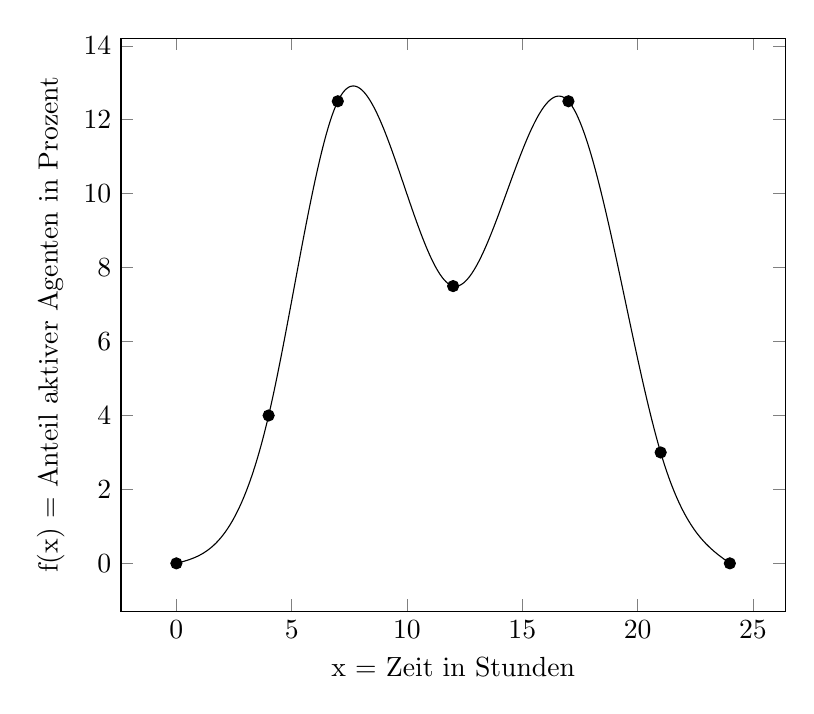
\begin{tikzpicture}
    \pgfplotsset{
        scale only axis,
    }

    \begin{axis}
        [
        xlabel={x = Zeit in Stunden},
        ylabel={f(x) = Anteil aktiver Agenten in Prozent},
        samples=100,
        ]
        \addplot [only marks] table {
            0 0
            4 4
            7 12.5
            12 7.5
            17 12.5
            21 3
            24 0
        };


        \addplot[][domain=0:4]{+0.05212125853316996*x^3+3.4e-60*x^2+0.1660598634692806*x^1+0*x^0};
        \addplot[][domain=4:7]{+-0.19010136076913603*x^3+2.9066714316276716*x^2+-11.460625863041406*x^1+15.502247635347583*x^0};
        \addplot[][domain=7:12]{+0.12557646303751677*x^3+-3.722562868312037*x^2+34.94401423653655*x^1+-92.77524593033432*x^0};
        \addplot[][domain=12:17]{+-0.11369945737791003*x^3+4.891370266643328*x^2+-68.42318338292783*x^1+320.6935445475232*x^0};
        \addplot[][domain=17:21]{+0.12176450638893752*x^3+-7.117291885465897*x^2+135.724073202929*x^1+-836.1409094389987*x^0};
        \addplot[][domain=21:24]{+-0.061541335226351856*x^3+4.430976136297334*x^2+-106.78955525409884*x^1+861.454489760196*x^0};
    \end{axis}
    \label{fig:interpolation-graph}
\end{tikzpicture}


Nun muss nur noch die Einwohnerdichte pro km\textsuperscript{2} angenähert werden, damit eine grobe Gesamtanzahl an Agenten sich ableiten lässt.
Das Statistikamt Nord, das für Schleswig-Holstein und Stadtteile Hamburgs Statistiken sammelt, hat in ihrem Bericht aus dem Jahr 2021 die Einwohnerdichte aller Stadtteile Hamburgs aufgelistet~\cite{SAHHSH2022}.
Der Simulationsort dieser Arbeit umfasst die folgenden Stadtteile: Neustadt, St. Georg, Hohenfelde, Uhlenhorst, Winterhude, Eppendorf, Harvestehude und Rotherbaum.
Für diese Stadtteile wird die Einwohnerdichte pro km\textsuperscript{2} ausgelesen:

\begin{table}
    \centering
    \begin{tabular}{||r|l||}
        \hline
        Stadtteil    & Einw.~je km\textsuperscript{2} \\\hline\hline
        Neustadt     & 5575                           \\\hline
        St. Georg    & 6291                           \\\hline
        Hohenfelde   & 8578                           \\\hline
        Uhlenhorst   & 8516                           \\\hline
        Winterhude   & 7499                           \\\hline
        Eppendorf    & 9193                           \\\hline
        Harvestehude & 8636                           \\\hline
        Harvestehude & 6253                           \\\hline\hline
        Gesamt       & 60.541                         \\\hline
    \end{tabular}
    \centering
    \caption{Die Einwohnerzahl pro km\textsuperscript{2} für die genannten Stadtviertel}
    \label{tab:citizen-per-district}
\end{table}

Es werden absichtlich aus dieser Statistik manche Agentengruppen nicht entfernt oder hinzugefügt, da keine genauen Statistiken dazu von der Stadt Hamburg gegeben oder bei der Recherche aufgefunden werden konnten zum Verwenden in dieser Arbeit.
Jene Gruppen umfassen, sind aber nicht beschränkt auf: Kinder, Eltern, die Zuhause auf Kindern aufpassen, Home-Office-Workers, Alte oder kranke Leute, Arbeitslose und noch mehr.
Diese müssten theoretisch gesehen aus den Statistiken entfernt werden, während folgende Menschengruppen zu der Statistik hinzugezählt werden müssten: Pendler aus anderen Städten, Pendler aus anderen Stadtvierteln, Privatpersonen mit mehr als einem Fahrtziel, Berufsfahrer wie zum Beispiel Taxis oder Lieferanten, Touristen und so weiter.
Der Einfachheit halber wurde also die durchschnittliche Einwohnerzahl der betroffenen Stadtviertel genommen, anstatt alle Umweltfaktoren aus der echten Welt einzubeziehen.

Mit der Gesamtmenge an Einwohnern pro km\textsuperscript{2} lässt sich der Durchschnitt aller für dieser Simulation relevanter Stadtteile berechnen, der dann mit der Gesamtfläche des Simulationsortes multipliziert die Gesamtanzahl an aktiven Agenten ergibt.
Der Flächeninhalt der Simulation ist mithilfe einer OpenStreetMap-Karte~\cite{OSF2004} berechenbar:

\begin{figure}[h]
    \centering
    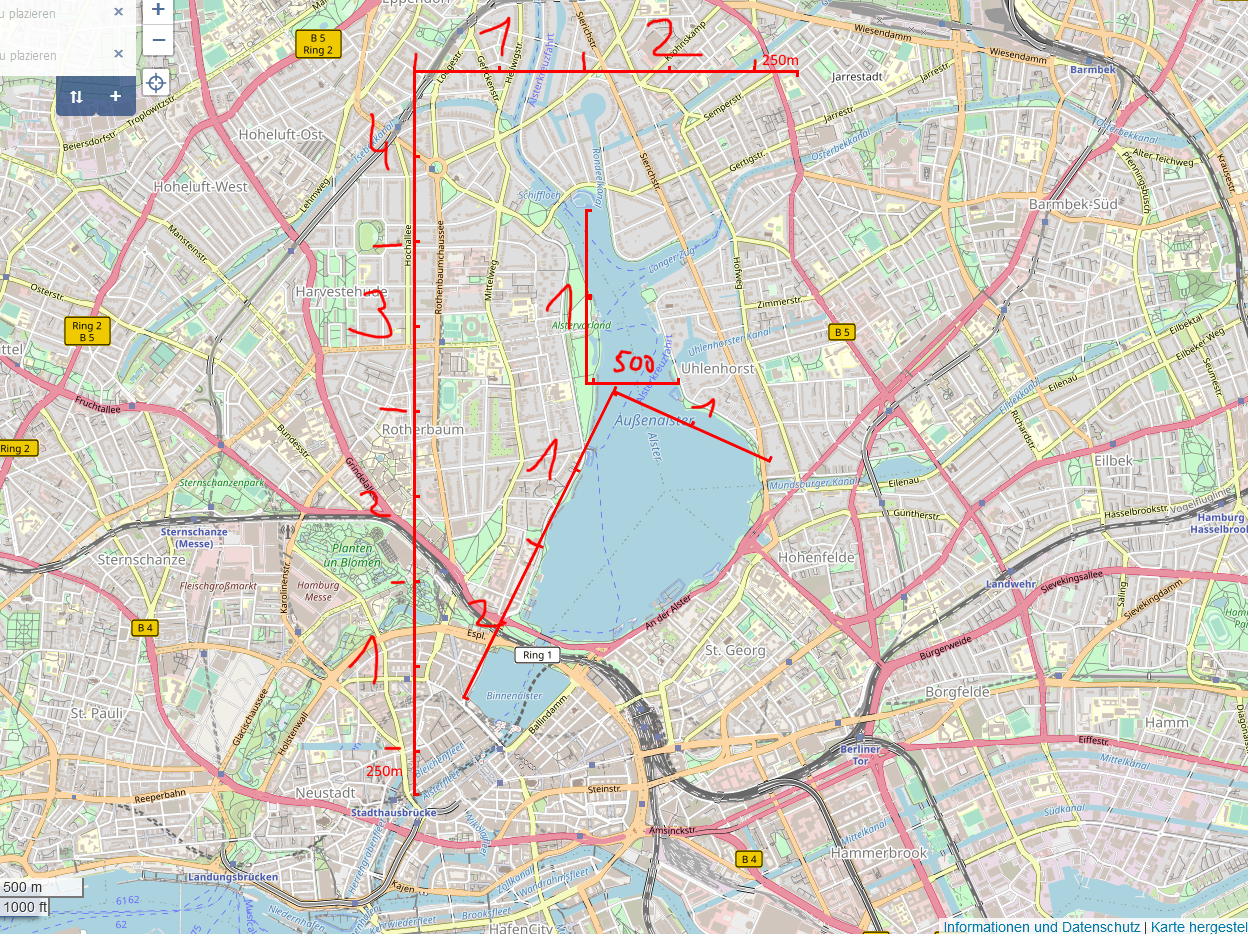
\includegraphics[width=0.75\textwidth]{calc-area}
    \caption{Grobe Flächenberechnung der bewohnbaren Bereiche}
    \label{fig:calc-area}
\end{figure}

Aus der Grafik~\ref{fig:calc-area} lassen sich folgende Flächen ablesen:

\begin{align}
    A &= (4,25~\unit{~km} * 2,25~\unit{~km}) - (0,5~\unit{~km}^2 + 2~\unit{~km}^2) \\
    &=  9,56~\unit{~km}^2 - 2,5~\unit{~km}^2 \\
    &=  7,06~\unit{~km}^2
\end{align}

Zuletzt wird noch die Multiplikation der durchschnittlichen Einwohnerdichte mit dem Flächeninhalt berechnet:

\begin{align}
    Gesamtanzahl Agenten &= 7,06~\unit{~km}^2 * ((60.541~\unit{~Einw~je~km}^2) / 8) \\
    &= 7,06~\unit{~km}^2 * (7.567,625~\unit{~Einw~je~km}^2) \\
    &= 53.427,4325~\unit{~Einw.} \\
    &\approx 53.427~\unit{~Einw.}
\end{align}

Angenäherte 53.427 Einwohner leben also in dem Gebiet um die Alster und sind täglich am Verkehr beteiligt.
Mit den Voraussetzungen lässt sich für jeden beliebigen Zeitpunkt an einem Arbeitstag eine Annäherung mit der Interpolationsgleichung~\ref{fig:interpolation} berechnen.
In der Simulation wird für jede Stunde, die neu angefangen wird, ein neuer Wert aus der Gleichung mit der durchschnittliche Einwohnerdichte multipliziert und damit als für diese Stunde, aktive Anzahl an Agenten festgelegt.
In dieser Simulation werden nur Daten für jede Stunde genommen, da der \code{BicycleLeader} ebenfalls nur jede Stunde einmal die Route fährt.
